% NOTE: Replace this self-contained article setup with the official CCAI workshop
% template from https://www.climatechange.ai/events/neurips2026 before submission.
% OpenReview: create the account immediately (CFP: creation can take up to 2 weeks).
\documentclass[10pt,twocolumn]{article}

\usepackage[margin=0.75in]{geometry}
\usepackage[T1]{fontenc}
\usepackage[utf8]{inputenc}
\usepackage{times}
\usepackage{microtype}
\usepackage{amsmath,amssymb}
\usepackage{booktabs}
\usepackage{array}
\usepackage{graphicx}
\usepackage[numbers,sort&compress]{natbib}
\usepackage[colorlinks=true,citecolor=blue,linkcolor=blue,urlcolor=blue]{hyperref}
\graphicspath{{figures/}}

\setlength{\columnsep}{0.23in}
\setlength{\textfloatsep}{8pt plus 2pt minus 2pt}
\setlength{\floatsep}{6pt plus 2pt minus 2pt}
\setlength{\abovecaptionskip}{4pt}
\setlength{\belowcaptionskip}{-2pt}

\title{Resource-Light Evaluation of Weather-Aware Vegetation Forecasting:\\
Simple Baselines, Frozen Encoders, and Sign Without Rate}
\author{Anonymous Submission}
\date{}

\begin{document}
\maketitle

\begin{abstract}
On 115 GreenEarthNet minicubes from tile 32UNU, a ridge read-out over frozen
Earth-observation embeddings plus weather predicts cube-mean NDVI 5--100 days
ahead, clearing a proxy climatology, an observation-process control, and a
permutation null while surviving a geographic block holdout. On paired
per-fold differences, however, no frozen encoder view---including
colour-infrared re-encodes---separably beats a 21-column summary of the same
bands at any horizon, and all nine are separably below it at 5 days. A
17-column baseline with current NDVI plus weather, and no image at all, beats
every frozen network at 5 and 25 days. A delta probe explains the split:
frozen representations recover the \emph{direction} of vegetation change, but
not its \emph{magnitude}. No frozen network beats persistence on both extreme
tails at any horizon, so pooled $R^2$ is the wrong operational metric for
drought and heat stress. Read as a handshake with EO-WM rather than a
contradiction, the result is a ground-up evaluation claim: state and sign are
already in the representation, while rate enters through the weather pathway.
\end{abstract}

\section{Introduction}
Short-horizon vegetation forecasts matter for climate adaptation because drought
and heat impacts are expressed locally in vegetation state before they appear
in coarse weather products. Operational services already think in multi-week
NDVI anomalies---for example early-drought products at 10/30/90-day leads and
Copernicus vegetation-stress indicators---and the decision is often binary at a
horizon: \emph{will this window fall below a vegetation-stress trigger at a
25-day lead?} That question is asked by drought monitoring desks, agricultural
and forestry analysts, and ecosystem observatories. It is also asked by model
builders who must decide whether a large frozen foundation model is worth the
compute when a small ridge might already answer it.

EarthNet2021 framed weather-conditioned Earth-surface forecasting as a guided
video task \citep{requena2021earthnet2021}; GreenEarthNet sharpened that framing
to high-resolution vegetation forecasting from Sentinel-2 and meteorology
\citep{benson2024greenearthnet}. The 2026 climate-AI agenda emphasises
ground-up, resource-aware evaluation: smaller or hybrid models, open tools, and
honest accounting of what signal is actually available. In that setting, the
central question is not whether a frozen vision encoder contains \emph{some}
signal. It is whether that signal adds climate-relevant skill beyond the
baselines a practitioner would deploy first---band statistics, current NDVI,
and weather---and whether pooled skill hides failure on the stress tails that
matter for adaptation.

We study that question with all encoders frozen and no new architecture. On 115
GreenEarthNet minicubes from tile 32UNU, ridge regression over frozen embeddings
plus weather predicts cube-mean NDVI 5--100 days ahead and clears every control
we test. Attribution does not follow. No frozen encoder separably beats a
band-matched hand-crafted baseline at any horizon, and current NDVI plus weather
alone beats every frozen network at 5 and 25 days. Companion probes show that
frozen appearance features carry the \emph{sign} of vegetation change but not
its \emph{rate}, and that weather explains only a within-season
\emph{proxy} fraction of the residual anomaly on this single-year tile. The
practical message is evaluative: for short-horizon vegetation monitoring, put
modelling effort into the weather pathway and into decision-oriented metrics,
rather than assume a larger frozen appearance backbone recovers severity.

\section{Related Work}
EarthNet2021 and GreenEarthNet established the benchmark setting we inherit
\citep{requena2021earthnet2021,benson2024greenearthnet}. EO-WM makes the weather
pathway explicit by decomposing forcing into climatology, anomalies, and
cumulative stress \citep{luo2026eowm}. The handshake with our study is
conceptual. EO-WM already separates direction-sensitive and amplitude-sensitive
diagnostics (DHR vs.\ DAE), reports a larger relative gain on direction than on
amplitude versus Wan2.1, and notes in its Table~5 that classifier-free guidance
can raise magnitude reproduction without improving ranking. We observe an
analogous split one stage upstream, before sequence modelling: frozen appearance
representations preserve the sign of vegetation change more readily than its
magnitude. We are not reproducing EO-WM's tables (different masks, they train,
we freeze, they predict pixels) and we do not treat their amplification setting
as the main result---they already declined to.

On the representation side we probe DINOv2 \citep{oquab2024dinov2} and
Satlas-pretrained remote-sensing encoders \citep{bastani2023satlaspretrain}.
The contribution is evaluative, not architectural: whether large pre-trained
features already contain the climate signal of interest more economically than
small band-statistics baselines and persistence/climatology controls.

\section{Setup}
\paragraph{Data and target.}
We use 115 GreenEarthNet minicubes from tile 32UNU, all from 2018. Each cube is
128\,$\times$\,128 pixels at 20\,m over an approximately 150-day window
\citep{benson2024greenearthnet}. The forecast target is cube-mean NDVI at
$\Delta \in \{5,25,50,100\}$ days. Tile 32UNU has no seasonal-split coverage, so
the leave-year-out climatology used elsewhere in the benchmark is not
computable here; weather ceilings on this tile are therefore
within-season \emph{proxies}, not H1.

\paragraph{Frozen predictors and baselines.}
Predictors are frozen EO/image encoders with a ridge read-out. We compare them
to a band-matched hand-crafted summary (\texttt{raw\_rgb\_only}; 21 columns of
the same RGB bands the networks receive) and to a 17-column autoregressive
baseline $[\mathrm{NDVI}(t),\mathrm{weather}]$ with no image. Full
\texttt{raw\_features} additionally sees all four bands and NDVI statistics; we
report it for context but do not treat it as a network. A multi-image Satlas
encoder is a positive control and is not single-image comparable (one embedding
can pool up to eight retained frames over a 0--105 day lookback).

\paragraph{Protocol.}
Evaluation is leakage-safe at the cube level (cube, LOCO, and spatial-block
splits); effective $n$ is counted in cubes. ``X beats Y'' uses paired per-fold
differences with a delete-one-fold jackknife, not overlapping marginal
intervals. A plausibility screen drops forecast rows that touch three
cloud-contaminated frames (midsummer cube-mean NDVI below zero at clear
fractions $0.59$--$0.63$) out of 1580 retained frames. Controls: persistence,
proxy climatology, observation-process, horizon-alone, and a permutation null.

\section{Results}
\subsection{Forecasting works; the representation is not the reason}
Table~\ref{tab:headline} summarises the Tier-1 forecast table. Skill is real:
the best rows reach $R^2=0.871/0.743/0.625/0.639$ at 5/25/50/100 days. The
observation control never exceeds $0.072$, the horizon-alone control is negative
at every horizon, and the permutation null sits near empirical zero. Encoder
rows remain positive under spatial blocking, even though the proxy climatology
collapses there.

\begin{table*}[t]
\centering
\small
\begin{tabular}{lcccc}
\toprule
Model row & 5 d & 25 d & 50 d & 100 d \\
\midrule
raw\_features + weather & $0.871$ & $0.743$ & $0.625$ & $0.639$ \\
raw\_rgb\_only + weather & $0.853$ & $0.727$ & $0.589$ & $0.556$ \\
$[\mathrm{NDVI}(t), \mathrm{weather}]$ only & $0.773$ & $0.693$ & $0.522$ & $0.406$ \\
best frozen network & $0.712$ & $0.670$ & $0.626$ & $0.586$ \\
\midrule
persistence & $0.690$ & $0.542$ & $0.124$ & $0.129$ \\
proxy climatology & $0.026$ & $0.125$ & $0.136$ & $-0.164$ \\
observation control & $0.014$ & $0.056$ & $0.072$ & $-0.024$ \\
horizon-only control & $-0.006$ & $-0.006$ & $-0.007$ & $-0.023$ \\
permutation null & $-0.014$ & $-0.002$ & $-0.007$ & $-0.024$ \\
\bottomrule
\end{tabular}
\caption{Headline pooled out-of-fold $R^2$ for cube-mean NDVI on 115 cubes
(tile 32UNU). Effective $n$ in cubes: 115/114/115/94. Nested-CV ridge, shared
$[\mathrm{NDVI}(t),\mathrm{weather}]$ base, plausibility screen on. ``Best
frozen network'' is the strongest of nine encoder views per horizon.}
\label{tab:headline}
\end{table*}

\begin{figure}[t]
\centering
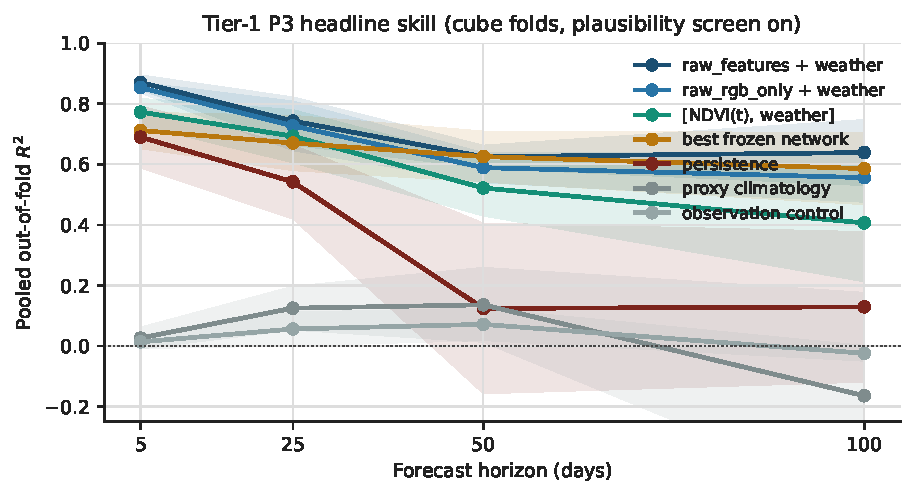
\includegraphics[width=\linewidth]{fig1_headline_r2.pdf}
\caption{Headline pooled $R^2$ versus horizon (Tier-1 P3, cube folds,
plausibility screen on). Shaded bands are delete-one-fold jackknife intervals.
Baselines and weather clear the observation and proxy-climatology controls;
the best frozen network stays below the band-matched hand-crafted row.}
\label{fig:headline}
\end{figure}

On paired per-fold differences, \emph{no} frozen encoder view separably beats
\texttt{raw\_rgb\_only} at any horizon (Figure~\ref{fig:paired}). At 5 days all
nine are separably \emph{below} it ($-0.141$ to $-0.267$). Colour-infrared twins
move some networks by at most $+0.14$ and never enough to reach the baseline.
The 17-column $[\mathrm{NDVI}(t),\mathrm{weather}]$ row beats every frozen
network at 5 and 25 days. For a drought desk that needs a short-lead answer,
that is the resource-aware default until a representation proves otherwise.

\begin{figure*}[t]
\centering
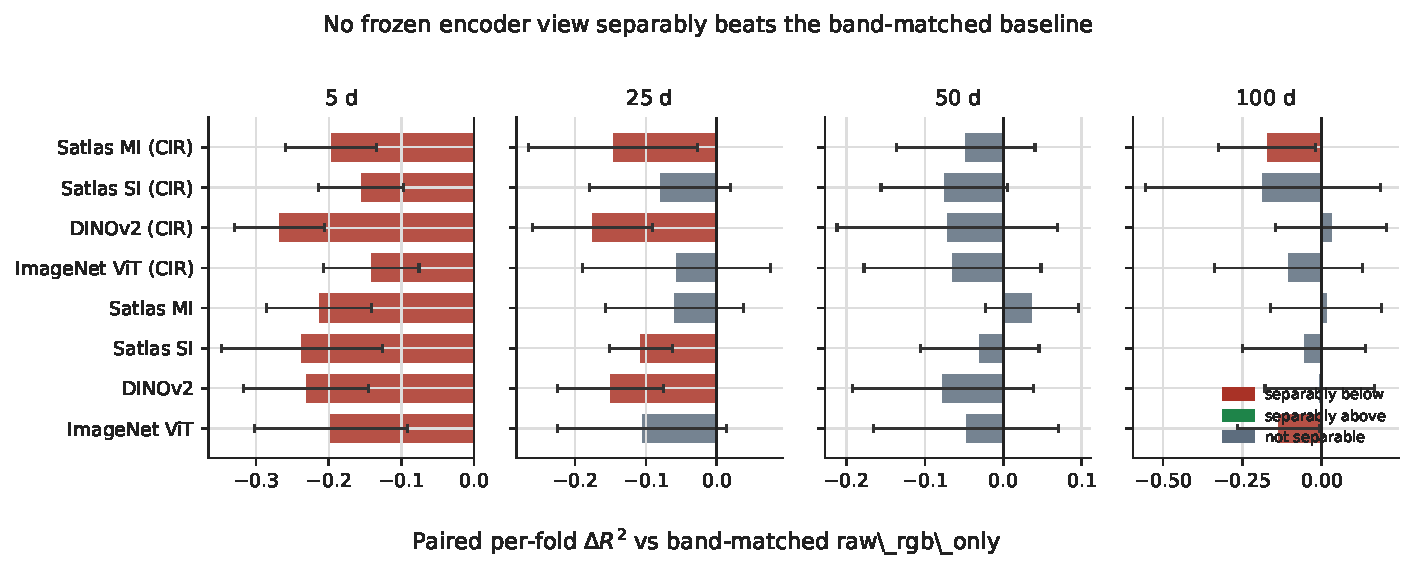
\includegraphics[width=\textwidth]{fig2_paired_vs_bandmatched.pdf}
\caption{Paired per-fold $\Delta R^2$ of each frozen encoder view against
band-matched \texttt{raw\_rgb\_only}. Red bars are separably below; no view is
separably above at any horizon.}
\label{fig:paired}
\end{figure*}

\subsection{Direction without rate; tails without pooled skill}
\begin{table}[t]
\centering
\footnotesize
\begin{tabular}{@{}>{\raggedright\arraybackslash}p{0.22\columnwidth}>{\raggedright\arraybackslash}p{0.70\columnwidth}@{}}
\toprule
Probe & Key measured result \\
\midrule
P2 sign & DINOv2: $\rho=0.606\,[0.546,0.665]$; margin $+0.54$ over the gap-length control. Band-matched \texttt{raw\_rgb\_only} reaches $0.695$. \\
P2 magnitude & No encoder recovers rate: all $\rho \leq 0.12$; 3 of 4 encoders flip margin sign across fold modes. \\
P4 proxy ceiling & Weather explains $0.130\,[0.063,0.197]$ (\texttt{cube}) and $0.085\,[0.007,0.162]$ (LOCO) of the within-season post-\emph{proxy}-climatology anomaly at \texttt{cell\_mean}/HGB; spatial blocking kills it. \\
\bottomrule
\end{tabular}
\caption{Companion probes. Frozen appearance features carry state and direction;
rate enters through the weather path. The P4 number is a proxy ceiling, not H1.}
\label{tab:crossprobe}
\end{table}

\begin{figure}[t]
\centering
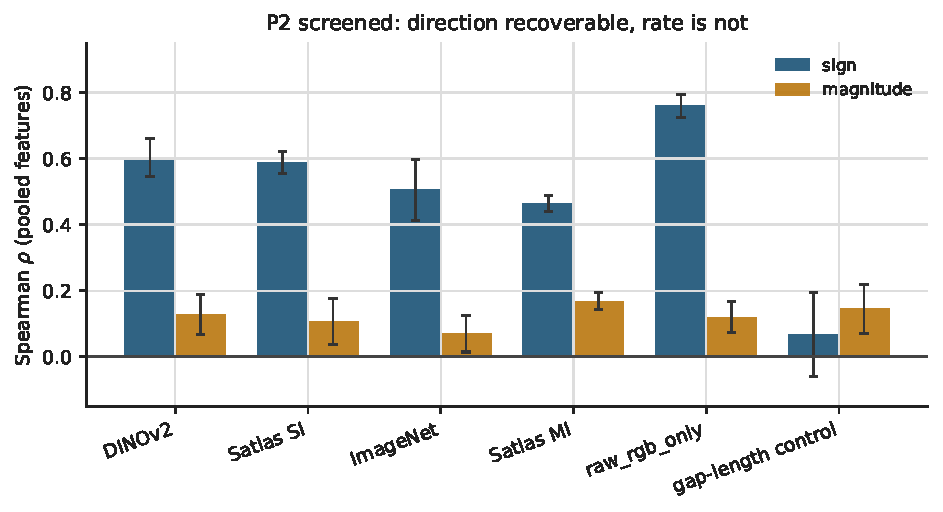
\includegraphics[width=\linewidth]{fig3_sign_vs_magnitude.pdf}
\caption{P2 screened cube-mean deltas (pooled features, linear read-out):
Spearman $\rho$ for sign versus magnitude. Direction clears the gap-length
control; rate does not.}
\label{fig:signmag}
\end{figure}

Table~\ref{tab:crossprobe} and Figure~\ref{fig:signmag} interpret the forecast.
Embedding deltas recover sign robustly but not magnitude---the same
dissociation EO-WM encodes in DHR versus DAE. Weather alone explains about
$0.09$--$0.13$ of the within-season residual anomaly on this tile. A
leave-year-out check on seasonal tile 30TVN is inconclusive (proxy $+0.192$
vs.\ real $-0.136$; intervals overlap because the crossed fold count clamps to
four years), so we do not quote Stage~B as H1.

\begin{table}[t]
\centering
\footnotesize
\begin{tabular}{lcccc}
\toprule
Skill vs.\ persistence & 5 d & 25 d & 50 d & 100 d \\
\midrule
\texttt{raw\_rgb\_only} / extreme\_low & $+0.12$ & $+0.30$ & $+0.50$ & $+0.69$ \\
\texttt{raw\_rgb\_only} / extreme\_high & $+0.75$ & $+0.38$ & $-0.72$ & $-0.57$ \\
DINOv2 / extreme\_low & $-1.31$ & $-0.51$ & $+0.34$ & $+0.68$ \\
DINOv2 / extreme\_high & $+0.35$ & $+0.29$ & $-0.31$ & $-0.62$ \\
\bottomrule
\end{tabular}
\caption{Decision-oriented diagnostic: skill against persistence in the
extreme tails (cube-mean, cube folds, Tier-1 protocol). No \emph{frozen
network} is positive on both \texttt{extreme\_low} and \texttt{extreme\_high}
at any horizon. Hand-crafted rows can clear both tails at short leads and still
fail on \texttt{extreme\_high} at 50--100\,d. This is a diagnostic for early
warning, not a claim of operational deployment.}
\label{tab:tails}
\end{table}

\begin{figure}[t]
\centering
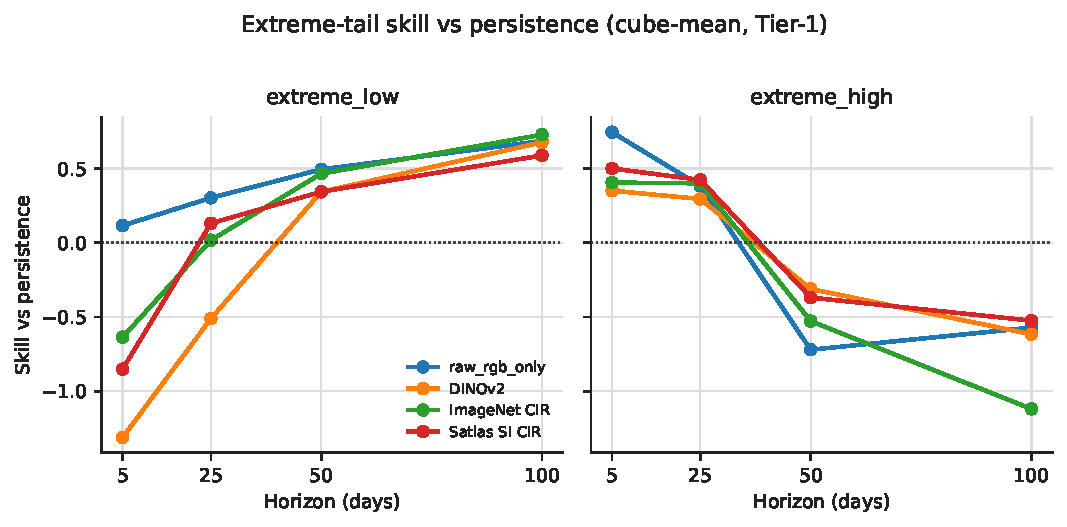
\includegraphics[width=\linewidth]{fig4_extreme_tails.pdf}
\caption{Skill against persistence in the extreme tails
(Table~\ref{tab:tails}). No frozen network is positive on both tails at any
horizon.}
\label{fig:tails}
\end{figure}

Table~\ref{tab:tails} and Figure~\ref{fig:tails} are the climate-facing reading
of the same predictions. Pooled $R^2$ lives in near-normal rows. On the extreme
subset, frozen networks are negative against persistence in
\texttt{extreme\_low} at 5--25 days, and no frozen network is positive on
\emph{both} extreme tails at any horizon. That is exactly the risk of sign
without rate for heat and drought: a model can look strong overall and still
miss severity on the windows an early-warning trigger would fire on.

\section{Implications and Limits}
The practical division of labour is simple. Use small, auditable baselines as
the first line for short-horizon vegetation-stress questions; require any frozen
encoder---or any world model---to beat $[\mathrm{NDVI}(t),\mathrm{weather}]$ and
to report sign and magnitude separately; put modelling capacity into the weather
pathway where physically meaningful stress can enter. That is a ground-up
evaluation recommendation, not an FM dunk.

Limits are real. This is one Alpine-foreland tile and one year; the weather
ceiling is a within-season proxy; Stage~B's second-order leak path remains
unquantified and is not quoted; P2/P4 are being re-aligned to the same
plausibility screen as P3; and we predict cube-mean NDVI, not pixels. These
limits argue for restraint and for a follow-on extreme-tile check on the 2018
heat/drought split---not for ignoring the result.

\section{Conclusion}
A resource-light read-out over Sentinel-2 plus E-OBS already forecasts
cube-mean NDVI well above climatology on GreenEarthNet. Frozen EO foundation
models are not, in this study, the reason. Direction of change is in the
pictures; rate is not; and the extreme tails do not follow the pooled headline.
That is useful climate-AI evidence: evaluate what is available before scaling
what is fashionable.

\bibliographystyle{plainnat}
\bibliography{refs}

\clearpage
\appendix
\section{Expanded Results}

\subsection{Full headline forecast table}
Table~\ref{tab:fullheadline} expands the main-text headline to all nine encoder
views from the Tier-1 re-run. The shared base is $[\mathrm{NDVI}(t),
\mathrm{weather}]$; all rows use ridge regression, cube folds, and the
plausibility screen.

\begin{table*}[h]
\centering
\small
\begin{tabular}{lcccc}
\toprule
Model row & 5 d & 25 d & 50 d & 100 d \\
\midrule
raw\_features + weather & $0.871$ & $0.743$ & $0.625$ & $0.639$ \\
raw\_rgb\_only + weather & $0.853$ & $0.727$ & $0.589$ & $0.556$ \\
$[\mathrm{NDVI}(t), \mathrm{weather}]$ only & $0.773$ & $0.693$ & $0.522$ & $0.406$ \\
imagenet\_vit\_b16\_cir & $0.712$ & $0.670$ & $0.524$ & $0.451$ \\
satlas\_s2\_swinb\_rgb\_cir & $0.698$ & $0.647$ & $0.514$ & $0.370$ \\
satlas\_s2\_swinb\_mi\_rgb & $0.640$ & $0.667$ & $0.626$ & $0.570$ \\
imagenet\_vit\_b16 & $0.656$ & $0.622$ & $0.542$ & $0.421$ \\
satlas\_s2\_swinb\_rgb & $0.616$ & $0.620$ & $0.559$ & $0.500$ \\
dinov2\_vitb14 & $0.622$ & $0.577$ & $0.512$ & $0.550$ \\
dinov2\_vitb14\_cir & $0.586$ & $0.551$ & $0.517$ & $0.586$ \\
\midrule
persistence & $0.690$ & $0.542$ & $0.124$ & $0.129$ \\
proxy climatology & $0.026$ & $0.125$ & $0.136$ & $-0.164$ \\
observation control & $0.014$ & $0.056$ & $0.072$ & $-0.024$ \\
permutation null & $-0.014$ & $-0.002$ & $-0.007$ & $-0.024$ \\
horizon-only control & $-0.006$ & $-0.006$ & $-0.007$ & $-0.023$ \\
\bottomrule
\end{tabular}
\caption{Tier-1 P3 headline table from the 115-cube re-run. Effective $n$ in
cubes is 115/114/115/94 at 5/25/50/100 days. The multi-image Satlas row is kept
for completeness but is not single-image comparable.}
\label{tab:fullheadline}
\end{table*}

\subsection{Protocol summary}
\begin{itemize}
\item \textbf{Data.} 115 GreenEarthNet minicubes from tile 32UNU, all from 2018.
\item \textbf{Forecast target.} Cube-mean NDVI at 5, 25, 50, and 100 days.
\item \textbf{Retained frames and rows.} 1580 retained frames in the rebuilt
manifest; 1540 total forecast rows in the Tier-1 run.
\item \textbf{Plausibility screen.} The shared target builder flags 3 of 1580
retained frames as implausible; removing any forecast row touching one of them
drops 8/5/5/0 rows at 5/25/50/100 days, changing row counts from
518/489/450/196 to 510/484/445/196.
\item \textbf{Cross-validation.} Cube-grouped splits only; claims are reported for
\texttt{cube}, LOCO, and \texttt{spatial\_block}. Effective sample size is
cubes, not frames.
\item \textbf{Comparisons.} ``X beats Y'' is always the paired per-fold difference
with a delete-one-fold jackknife interval, not a comparison of overlapping
marginal confidence intervals.
\item \textbf{Controls.} Persistence, proxy climatology, observation-process,
horizon-only, and permutation controls travel with the main table. P4 also
includes a day-of-year sanity control.
\end{itemize}

\subsection{Paired separability and colour-infrared twins}
\begin{table}[h]
\centering
\footnotesize
\begin{tabular}{@{}>{\raggedright\arraybackslash}p{0.21\columnwidth}>{\raggedright\arraybackslash}p{0.71\columnwidth}@{}}
\toprule
Question & Measured answer \\
\midrule
Do frozen encoders beat the band-matched baseline? & No. At 5 days all 9 encoder views are separably below \texttt{raw\_rgb\_only} by $-0.141$ to $-0.267$; at 25 days 4 of 9 are separably below; at 50 days none is separable either way; at 100 days 3 of 9 are separably below and none above. \\
Does NIR access rescue the frozen networks? & No. Across RGB/CIR twins, 16 of 48 comparisons are separable and 22 of 48 have the CIR row ahead at all. Gains of $+0.05$ to $+0.14$ appear mainly at 5 and 25 days for two single-image encoders, but never enough to reach the band-matched baseline. \\
\bottomrule
\end{tabular}
\caption{Appendix summary of the paired tests that underpin the main claim.}
\label{tab:paired}
\end{table}

\subsection{Cross-probe handshake}
\begin{table}[h]
\centering
\footnotesize
\begin{tabular}{@{}>{\raggedright\arraybackslash}p{0.19\columnwidth}>{\raggedright\arraybackslash}p{0.73\columnwidth}@{}}
\toprule
Probe & Key number used in the paper \\
\midrule
P2 sign & DINOv2 reaches $\rho=0.606\,[0.546,0.665]$; the band-matched \texttt{raw\_rgb\_only} row reaches $0.695$, above every network. \\
P2 magnitude & All correlations are at most $0.12$; margins are at most $+0.07$; 3 of 4 encoders flip margin sign across fold modes. \\
P4 proxy ceiling & At \texttt{cell\_mean} under HGB, weather explains $0.130\,[0.063,0.197]$ on \texttt{cube} and $0.085\,[0.007,0.162]$ on LOCO; 17 of 54 weather rows exclude zero at 115 cubes. \\
\bottomrule
\end{tabular}
\caption{Numbers from the complementary probes used to interpret the main forecast result.}
\label{tab:handshake}
\end{table}

\subsection{Extreme-subset finding (Tier-1 screened table)}
The main forecast headline is dominated by near-normal rows. On the extreme
subset, under the Tier-1 protocol (nested-CV ridge, shared base, screen on):
\begin{itemize}
\item At 5 and 25 days, every \emph{frozen network} is negative against
persistence in \texttt{extreme\_low}.
\item At 50 and 100 days, networks turn positive on \texttt{extreme\_low} but
remain negative on \texttt{extreme\_high} (DINOv2 reaches $-0.62$ at 100\,d).
\item No frozen network is positive on \emph{both} extreme tails at any horizon.
\item Hand-crafted \texttt{raw\_rgb\_only} clears both tails at 5 and 25\,d
($+0.12/+0.75$ and $+0.30/+0.38$) and still fails on \texttt{extreme\_high} at
50--100\,d ($-0.72$, $-0.57$).
\end{itemize}

This is why the paper treats sign-versus-magnitude---and tail skill versus
pooled $R^2$---as climate-relevant rather than merely diagnostic: a model can
look strong overall and still miss the windows an early-warning trigger would
fire on.

\subsection{Proxy climatology check (30TVN)}
On seasonal tile 30TVN (87 cubes), Stage~A proxy weather skill is
$+0.192\,[+0.139,+0.245]$ while Stage~B leave-year-out skill is
$-0.136\,[-0.852,+0.581]$. The point estimates differ by $0.328$; the intervals
overlap because \texttt{crossed} folds clamp to four years. That is
\emph{not} evidence the proxy is sound---it is the absence of evidence either
way---and no H1-style number is quoted from Stage~B.

\subsection{Plausibility-screen alignment}
P3 applies \texttt{frame\_plausible} (in-season cube-mean NDVI below $0.15$
flagged as cloud). Screening 8 of 518 forecast rows at $\Delta=5$\,d moved
persistence from $+0.169$ to $+0.690$. P2 and P4 inherit the same opt-in flag;
screened CSVs are written beside the cubes as
\texttt{p2\_screened\_results.csv} / \texttt{p4\_screened\_results.csv} so the
published unscreened tables remain reproducible.


\end{document}
